\documentclass[final]{beamer}

% Packages
\usepackage[scale=1.24]{beamerposter}
\usepackage{graphicx}
\usepackage{booktabs}
\usepackage{amssymb}
\usepackage{amsmath}
%\usepackage{minted}
\usepackage{listings}
\usepackage{xcolor}
\usepackage{url}


\definecolor{darkgreen}{rgb}{0,0.6,0}
\lstdefinestyle{Python}{
    language        = Python,
    basicstyle      = \ttfamily,
    keywordstyle    = \color{blue},
    keywordstyle    = [2] \color{teal}, % just to check that it works
    stringstyle     = \color{green},
    commentstyle    = \color{darkgreen}\ttfamily
}

% Styling
\newcommand{\agsNote}[1]{\textcolor{cyan}{#1}}
\newcommand{\bfCenter}[1]{\centerline{\textbf{#1}}}
\usetheme{confposter}
\setbeamercolor{block title}{fg=red,bg=white}
\setbeamercolor{title}{fg=red,bg=white}
\setbeamercolor{block body}{fg=black,bg=white}
\setbeamercolor{block alerted title}{fg=white,bg=red}
\setbeamercolor{block alerted body}{fg=black,bg=white}
\setbeamercolor{block alerted title}{fg=red,bg=black!5}


% Formatting
\newlength{\sepwid}
\newlength{\onecolwid}
\newlength{\twocolwid}
\newlength{\threecolwid}
\setlength{\paperwidth}{48in}
\setlength{\paperheight}{36in}
\setlength{\sepwid}{0.024\paperwidth}
\setlength{\onecolwid}{0.22\paperwidth}
\setlength{\twocolwid}{0.464\paperwidth}
\setlength{\threecolwid}{0.708\paperwidth}
\setlength{\topmargin}{-0.5in}

\newcommand{\dif}{\mathrm{d}}

% Meta Data
\title{Community Supported Quasi-Monte Carlo (QMC) Software}
\author{Aleksei Sorokin (asorokin@hawk.iit.edu)\inst{1}, Sou-Cheng Choi\inst{1,2}, \\Michael McCourt\inst{3}, Jagadeeswaran Rathinavel\inst{1},
Fred Hickernell (hickernell@iit.edu)\inst{1}}
\institute[shortinst]{\inst{1} Illinois Institute of Technology,
                      \inst{2} Kamakura Corporation, 
                      \inst{3} SigOpt
                      }


% Headline
\setbeamertemplate{headline}{
 \leavevmode
  \begin{columns}[T]
    \vspace{.5in}
    %
    \hspace{.5in} 
    \begin{column}{.1\linewidth}
        \vskip1cm
        \hskip1cm
        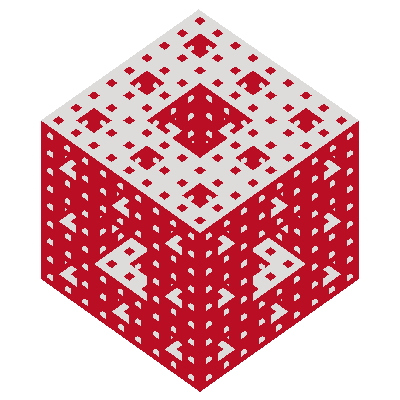
\includegraphics[width=.9\linewidth]{Images/IIT_Logo.jpg}
    \end{column}
    %
    \hspace{1in}
    \begin{column}{.8\linewidth}
         \vskip2cm
         \centering
         \usebeamercolor{title in headline}{\color{red}\Huge{\textbf{\inserttitle}}\\[0.5ex]}
         \usebeamercolor{author in headline}{\color{black}\Large{\insertauthor}\\[1ex]}
         \usebeamercolor{institute in headline}{\color{black}\Large{\insertinstitute}\\[1ex]}
         \vskip1cm
        \end{column}
\hspace{-2.5in}
    \begin{column}{.1\linewidth} 
        %\vskip1cm
         
\includegraphics[width=.75\linewidth]{Images/kamakura_logo.jpeg}
        \hskip1cm
    \end{column}     
    %
	\hspace{-1in}
        \begin{column}{.1\linewidth} 
        \vskip1cm
        
\includegraphics[width=.65\linewidth]{Images/SigOpt_Logo.png}
        \hskip1cm
    \end{column}           
   \vspace{1cm}
  \end{columns}
 \vspace{-0.1in}
 \hspace{0.5in}\begin{beamercolorbox}[wd=47in,colsep=0.15cm]{cboxb}\end{beamercolorbox}
 \vspace{0.1in}
}

\begin{document}
% Setup Format and Styling
\addtobeamertemplate{block end}{}{\vspace*{2ex}}
\addtobeamertemplate{block alerted end}{}{\vspace*{2ex}}
\setlength{\belowcaptionskip}{2ex}
\setlength\belowdisplayshortskip{2ex}
\begin{frame}[t]
\begin{columns}[t]

% Column 1
\begin{column}{\sepwid}\end{column}

\begin{column}{\onecolwid}\vspace{-.25in}

%    Software Objectives
\begin{block}{Software Objectives}
    To provide QMC software that is: 
    \begin{itemize}
        \item Comprised of free open source tools
        \item Easy to use for non-experts
        \item The recognized standard
    \end{itemize}
\end{block}

%    The QMC Problem
\begin{block}{The QMC Problem}
    
    \vspace{.25in}
    \bfCenter{Original Form} 
        \begin{equation*}
            \mu = \int_{T} g(t) \, \lambda(\dif t) 
            \label{eq:ogProblem}
        \end{equation*}
        $ g:T \rightarrow \mathbb{R} = $ original integrand \\
        $ \lambda = $ original measure
    \vspace{.5in}      
    
    \bfCenter{Convenient Form}
        \begin{equation*}
            \mu = \int_{X} f(x)\rho(x)dx = \int_{X} f(x) \, \nu( \dif x)
            \label{convForm}
        \end{equation*}
        $\nu = $ well defined probability measure\\
        $\phi: X \rightarrow T = $ change of variables\\
        $f: X \rightarrow \mathbb{R} $ = integrand after change of variables
    \vspace{.5in}
    
    
    \bfCenter{(Quasi-)Monte Carlo Approximation}
        \begin{equation*}
            \hat{\mu}_n = a_n \sum_{i=1}^{n} f(x_i)w_i =  \int_{X} f(x) \, \hat{\nu}( \dif x)
            \label{qmcApprox}
        \end{equation*}
        \begin{align*}
            \nu \approx \hat{\nu}_n & = a_n \sum_{i=1}^n w_i \delta_{\hat{x_i}}(\cdot) \\
            & = \text{discrete probability measure}
        \end{align*}
\end{block}

%    Design Challenges
\vspace{-.25in}
\begin{block}{Design Challenges}
    \begin{itemize}
        \item Atomize Monte Carlo method into objects
        \item Define abstract methods and properties
        \item Unify existing components into framework
        \item Expand framework to allow multi-level problems
        \item Develop thorough documentation 
        \item Ensure reproducibility
    \end{itemize}
\end{block}
\end{column}

\begin{column}{\onecolwid}\vspace{-.25in}

% Keister Example
\begin{block}{Keister Example}
\lstinputlisting[style=Python]{python/keister.py}
\end{block}

%    Stopping Criterion
\vspace{-.1in}
\begin{alertblock}{Stopping Criterion}
    Determine $n$ such that $\left | \mu - \hat{\mu}_n \right  | \leq \epsilon$
    \begin{itemize}
        \item Central Limit Theorem (CLT)
        \item CLT Repeated
        \item Mean Monte Carlo (Guaranteed)
        \item Lattice Cubature (Guaranteed)
    \end{itemize}
\end{alertblock}

%    Integrand
\vspace{-.1in}
\begin{alertblock}{Integrand}
    Specify and generate values $f(\hat{x})$ for $\hat{x} \in \hat{\nu}$
    \begin{itemize}
        \item Keister
        \item Asian Call
    \end{itemize}
\end{alertblock}

%    True Measure
\vspace{-.1in}
\begin{alertblock}{True Measure}
    Specify components of a general sampling method
    \begin{itemize}
        \item Uniform
        \item Gaussian
        \item Brownian Motion 
        \item Lebesgue
    \end{itemize}
\end{alertblock}

%    Discrete Distribution
\vspace{-.1in}
\begin{alertblock}{Discrete Distribution}
    Specify and generate $a_n \sum_{i=1}^n w_i \delta_{\hat{x_i}}(\cdot)$
    \begin{itemize}
        \item IID Standard Uniform
        \item IID Standard Gaussian
        \item Lattice
        \item Sobol
    \end{itemize}
\end{alertblock}

\end{column}


\begin{column}{\sepwid}\end{column}
\begin{column}{\twocolwid}\vspace{-.25in}

% Discrete Distributions Mimicking Measures
\begin{block}{Discrete Distributions Transformed to Mimic $\mathcal{N}_2(0,1)$}
    \begin{figure}
        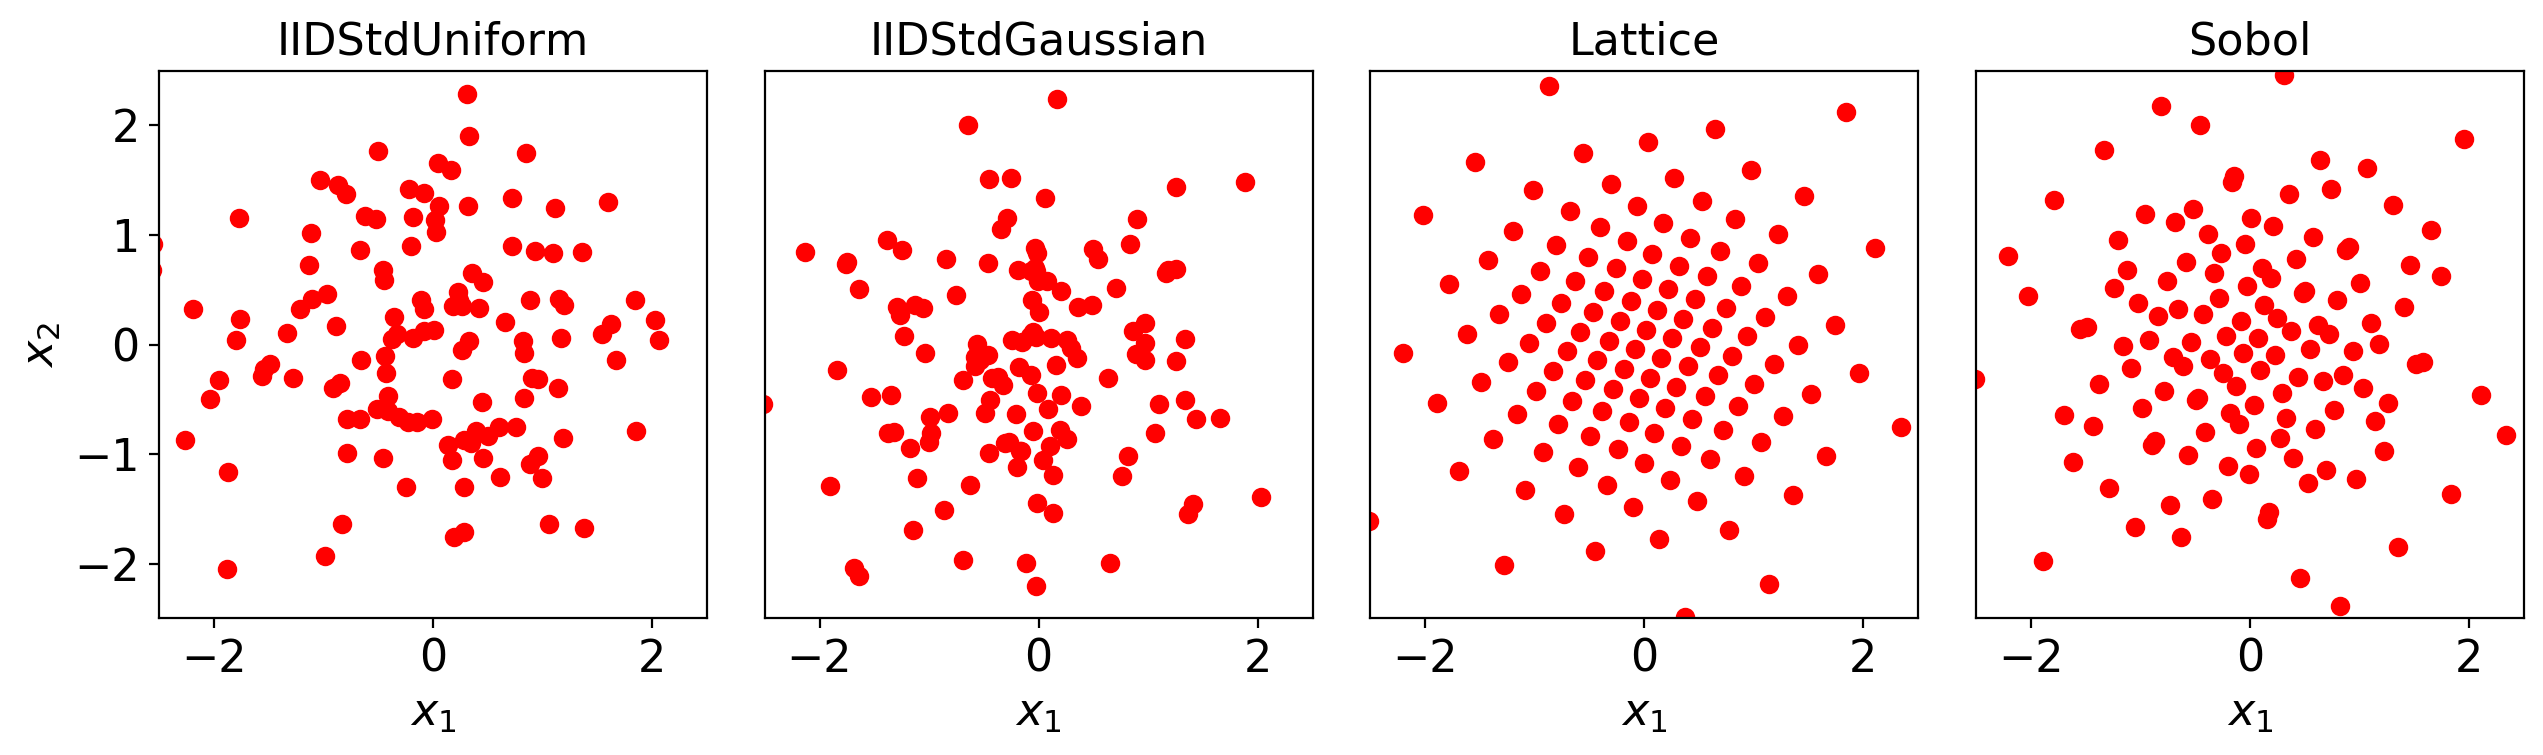
\includegraphics[width=1\textwidth]{Images/Gaussian_tm_transform.png}
    \end{figure}
    \bfCenter{\lstinputlisting[style=Python]{python/gaussian_sobol.py}}
\end{block}

% Stopping Criterion Comparison
%\vspace{-.25in}
\begin{block}{Stopping Criterion Comparison on Keister Example}
    %\bfCenter{Integration Time Comparison}
    \begin{figure}
        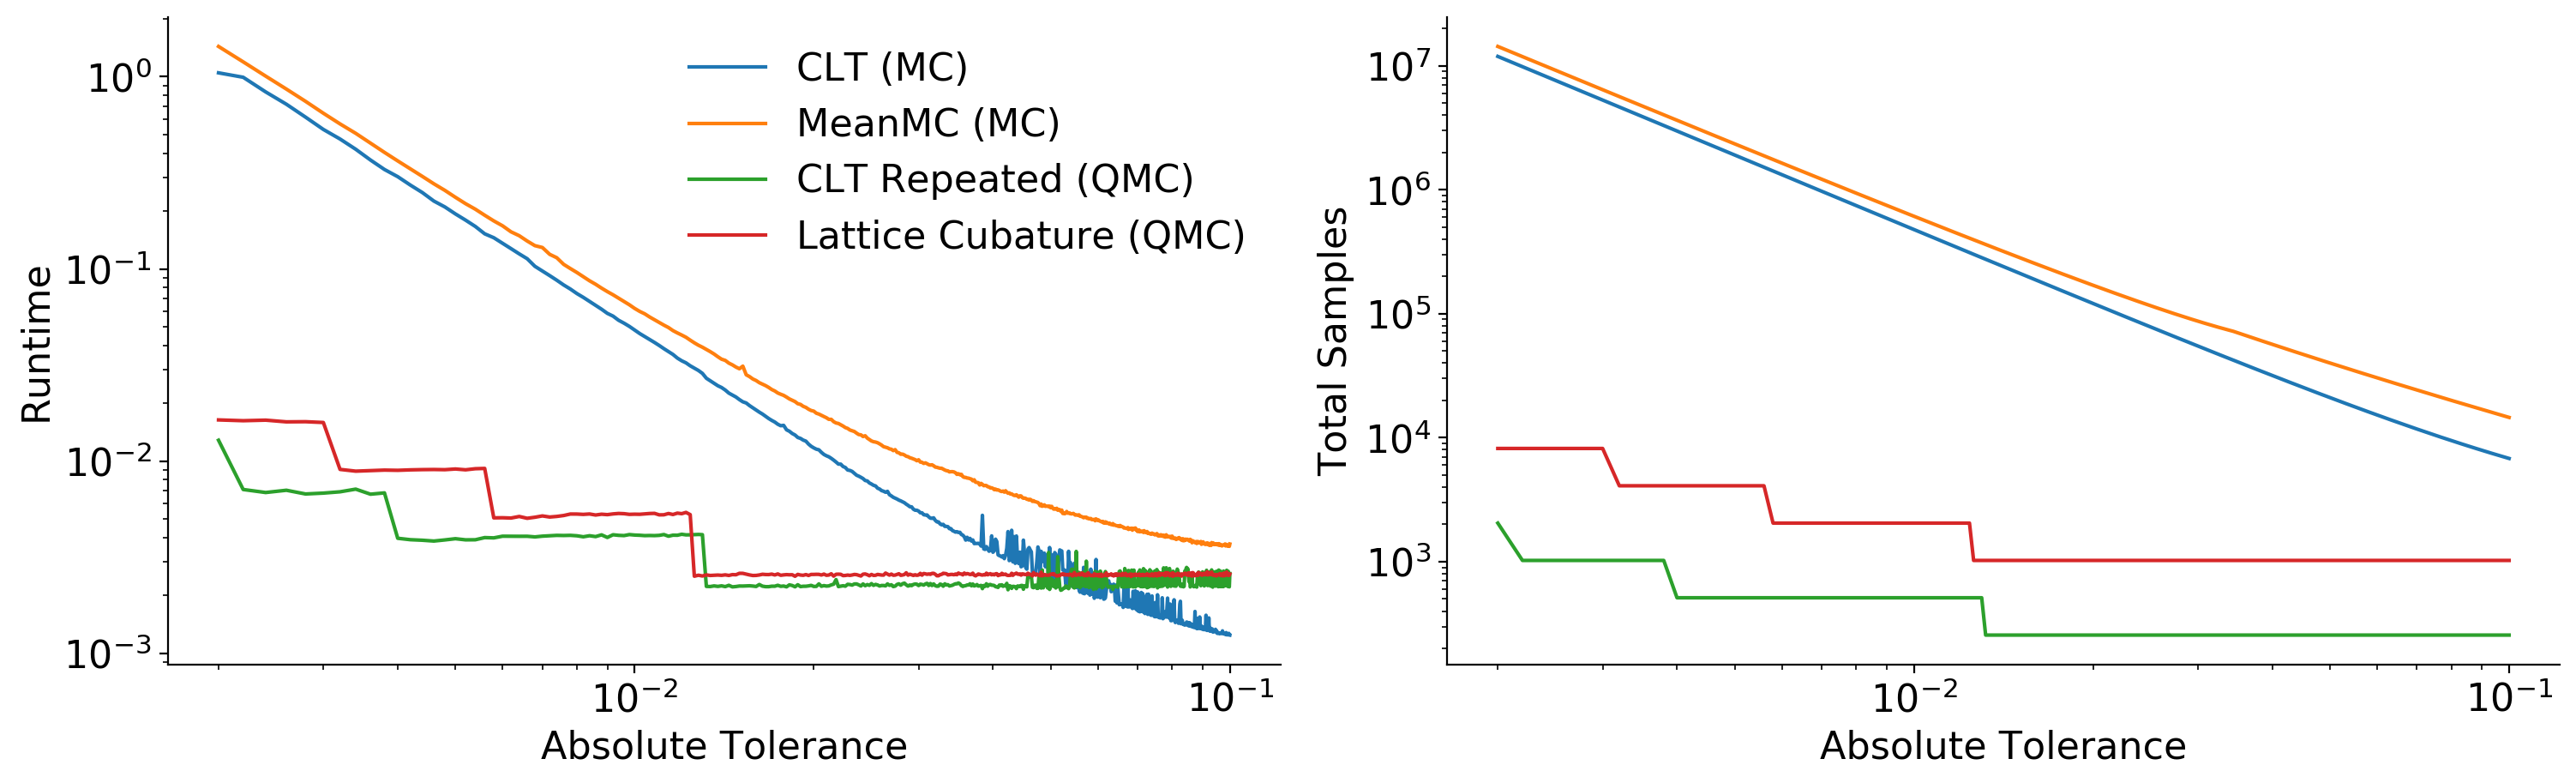
\includegraphics[width=1\textwidth]{Images/vary_abs_tol.png}
        %\caption{Multi-dimensional Asian Call Option integrated with respect to  Brownian Motion}
    \end{figure}
\end{block}

%\end{columns}

\begin{columns}[t,totalwidth=\twocolwid]  

\begin{column}{\onecolwid}\vspace{-1in}
%    Future Work 
%\vspace{-.25in}
\begin{block}{Future Work}
    \begin{itemize}
        \item Expand library of examples
        \item Incorporate established research packages
        \item Grow community of contributors
        \item Utilize community feedback to improve software
    \end{itemize}
\end{block}

% Acknowledgements
%\vspace{.5in}
\begin{block}{Acknowledgements}
    \begin{itemize}
        \item Thank you to SigOpt for continued funding and development support.
        \item Thank you to Dirk Nuyens for providing lattice and Sobol generators. 
    \end{itemize}
\end{block}

\end{column}

\begin{column}{\onecolwid}\vspace{-1in}

% References
%\vspace{-.25in}
\begin{block}{References}
\begin{itemize}
    \item \textbf{\url{https://github.com/QMCSoftware/QMCSoftware}}
    
    \item S.-C.~T.~Choi, Y.~Ding, F. J.~Hickernell, L.~Jiang,
    Ll.~A.~Jim\'enez Rugama, D.~Li, R.~Jagadeeswaran, X.~Tong, K.~Zhang, Y.~Zhang, and X.~Zhou, ``GAIL: Guaranteed Automatic Integration Library (versions 1.0-2.3),'' MATLAB software, 2013-2019.
    \url{http://gailgithub.github.io/GAIL\_Dev/}
    
    \item F.~Y.~Kuo and D.~Nuyens, ``Application of quasi-Monte Carlo methods to elliptic PDEs with random diffusion coefficients -- a survey of analysis and implementation,'' Foundations of Computational Mathematics, 16(6):1631-1696, 2016.
\end{itemize}
\end{block}

\end{column}
\end{columns}

\end{column}

\end{columns}



\end{frame}
\end{document}
